%
% $RCSfile: knowledge_designer.tex,v $
%
% Copyright (C) 2002-2008. Christian Heller.
%
% Permission is granted to copy, distribute and/or modify this document
% under the terms of the GNU Free Documentation License, Version 1.1 or
% any later version published by the Free Software Foundation; with no
% Invariant Sections, with no Front-Cover Texts and with no Back-Cover
% Texts. A copy of the license is included in the section entitled
% "GNU Free Documentation License".
%
% http://www.cybop.net
% - Cybernetics Oriented Programming -
%
% http://www.resmedicinae.org
% - Information in Medicine -
%
% Version: $Revision: 1.1 $ $Date: 2008-08-19 20:41:07 $ $Author: christian $
% Authors: Christian Heller <christian.heller@tuxtax.de>
%

\subsection{Knowledge Designer}
\label{knowledge_designer_heading}
\index{CYBOL Knowledge Designer}
\index{Unified Modeling Language}
\index{UML}
\index{CYBOL Template Diagram}
\index{TD}
\index{CYBOL Model Diagram}
\index{MD}
\index{CYBOL Organisation Diagram}
\index{OD}
\index{CYBOL Communication Diagram}
\index{CD}

Section \ref{unified_modeling_language_heading} classified diagrams of the
\emph{Unified Modeling Language} (UML) notation into \emph{Structure},
\emph{Behaviour} and \emph{Interaction}. With interaction- being a subset of
behaviour diagrams, there are actually just \emph{two} main categories for UML
diagram classification: \emph{Structure} and \emph{Behaviour}. Since the idea
underlying \emph{this} work is to look at systems from two perspectives
(section \ref{approach_heading}): \emph{Statics} and \emph{Dynamics}, whereby
the former gets split up into two further perspectives: \emph{States} and
\emph{Logic}, the question arises whether or not UML diagrams could be
categorised accordingly? The answer is: \emph{Not quite.} There are a number of
aspects that have to be considered:

\begin{itemize}
    \item[-] UML classes bundle state- and logic aspects (attributes and
        methods). A CsD does not only express the relations between attributes,
        but also those between methods. This fact makes it impossible to sort
        that diagram into just one of the categories: state or logic. Likewise
        does an SD, to take a second example, not just display the order of
        message calls, but also their bundling with objects. CYBOL templates,
        on the other hand, strictly separate state- and logic knowledge.
    \item[-] Classes in a CsD are linked network-like and may have bidirectional
        relations. Composition (recursion) as concept is missing in the class
        element of the UML meta model. The CYBOP knowledge schema is innately
        hierarchical and uses solely unidirectional relations.
    \item[-] UML objects (instances) know from which class (type) they stem from.
        Not at least, this is necessary for mechanisms like polymorphism (based
        on runtime inheritance) to work. CYBOL models know nothing about the
        original template they were initialised with; any links to it are lost.
\end{itemize}

However, an attempt will now be made to categorise the UML diagrams accordingly:

\begin{itemize}
    \item \emph{Statics (States):} CsD
    \item \emph{Statics (Logic):} SMD, AD, SD, TiD, CoD, IOD, UCD
    \item \emph{Dynamics:} ObD, CSD
    \item \emph{Others:} CmD, PD, DD
\end{itemize}

All diagrams formerly belonging to either \emph{Behaviour} or \emph{Interaction},
are now summed up in the \emph{Statics (Logic)} category. Former \emph{Structure}
diagrams are split up into the one describing \emph{Statics (States)} and those
illustrating \emph{Dynamics} (runtime aspects). Some diagrams dealing with issues
like packaging or distribution are put into an extra category called \emph{Others}.

Because of the different programming philosophy behind CYBOP, standard UML
diagrams cannot be used unalteredly for the design of CYBOL applications. Some
of them, however, could be quite useful, when adapted a bit. The \emph{Importance}
column in table \ref{diagrams_table} indicated that not all diagram types are
really needed to effectively design a system. For creating CYBOL applications,
the following four can be considered sufficient. They model the structure of:

\begin{enumerate}
    \item \emph{Template Diagram} (TD): one design-time template (hierarchical,
        ontological concept), with purely unidirectional relations; does not
        illustrate relations between different concepts, as these are only
        established by logic models at runtime; could look like CsD or a tree,
        only that a template may not only represent states, but also logic
        (algorithms, workflows) (figure \ref{td_figure})
    \item \emph{Model Diagram} (MD): the runtime model tree; comparable to ObD,
        but a simple tree with named nodes would suffice; is important because
        input/ output parameters of operations are given as dot-separated paths
        to runtime knowledge tree models (figure \ref{md_figure})
    \item \emph{Organisation Diagram} (OD): template directories; could look
        like CmD or PD or a simple tree (figure \ref{od_figure})
    \item \emph{Communication Diagram} (CD): a network of communicating
        systems, which may run on the same or on different physical machines
        (nodes); could look like DD; not to be mixed up with UML CoD (figure
        \ref{cd_figure})
\end{enumerate}

\begin{figure}[ht]
    \begin{center}
        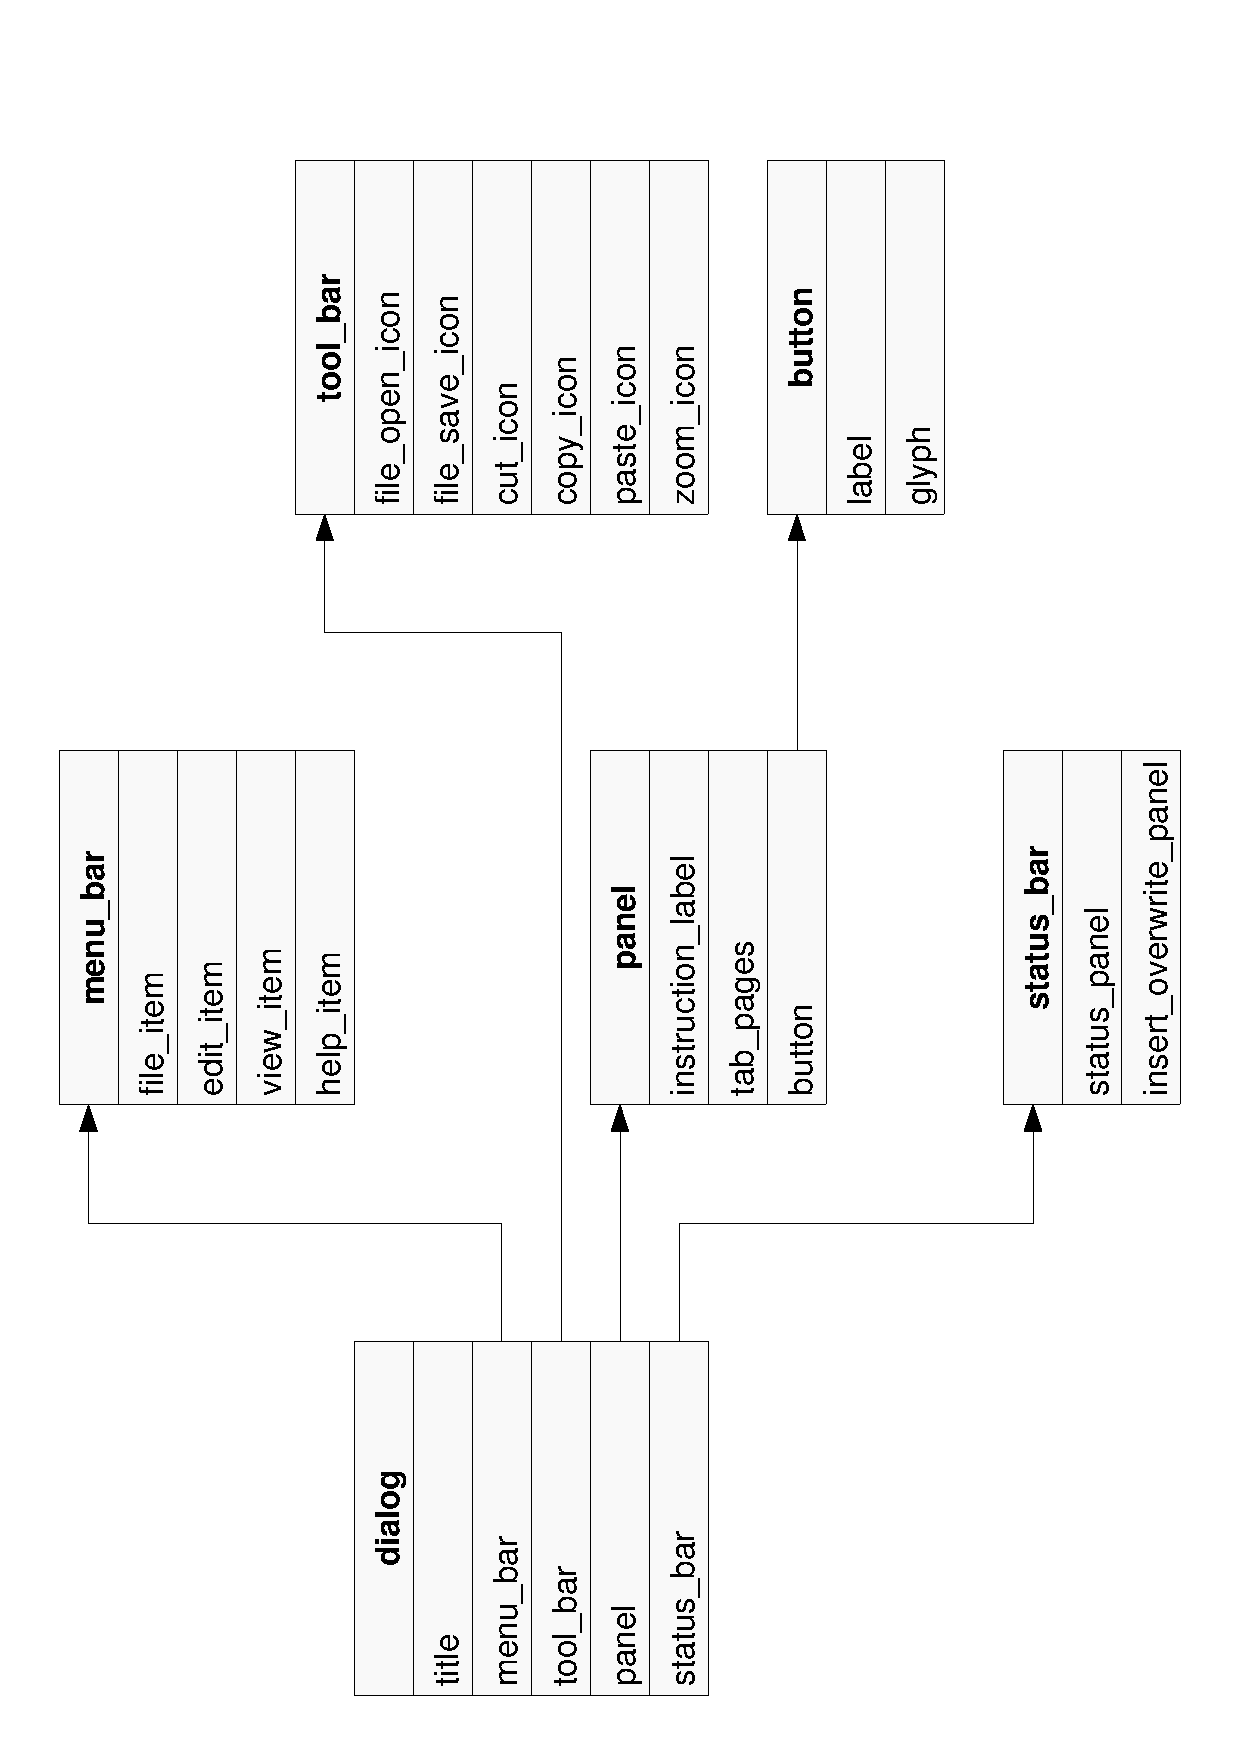
\includegraphics[scale=0.3,angle=-90]{graphic/td.pdf}
        \caption{CYBOL Template Diagram (TD) Proposal}
        \label{td_figure}
    \end{center}
\end{figure}

As said above, the four diagrams may look similar to their corresponding UML
pendant. For demonstration reasons, one possible proposal is given for each
diagram type. The TD (figure \ref{td_figure}) illustrates the same graphical
dialogue that was shown in the \emph{Template Editor} (figure
\ref{editor_figure}), in the previous section. The diagram looks pretty similar
to a UML CsD. Attributes and methods are not bundled in one concept though, and
inheritance does not exist. Associations are drawn if a concept links to an
external concept which may reside in another file (like the \emph{menu\_bar}),
for example. If a part (like the \emph{title}) is hold inline in the concept,
on the other hand, an association is not displayed. Upon clicking on a part in
a concept box, a dialogue opens up that allows the entry of meta data like the
part's channel, abstraction, model and further properties (details).

\begin{figure}[ht]
    \begin{center}
        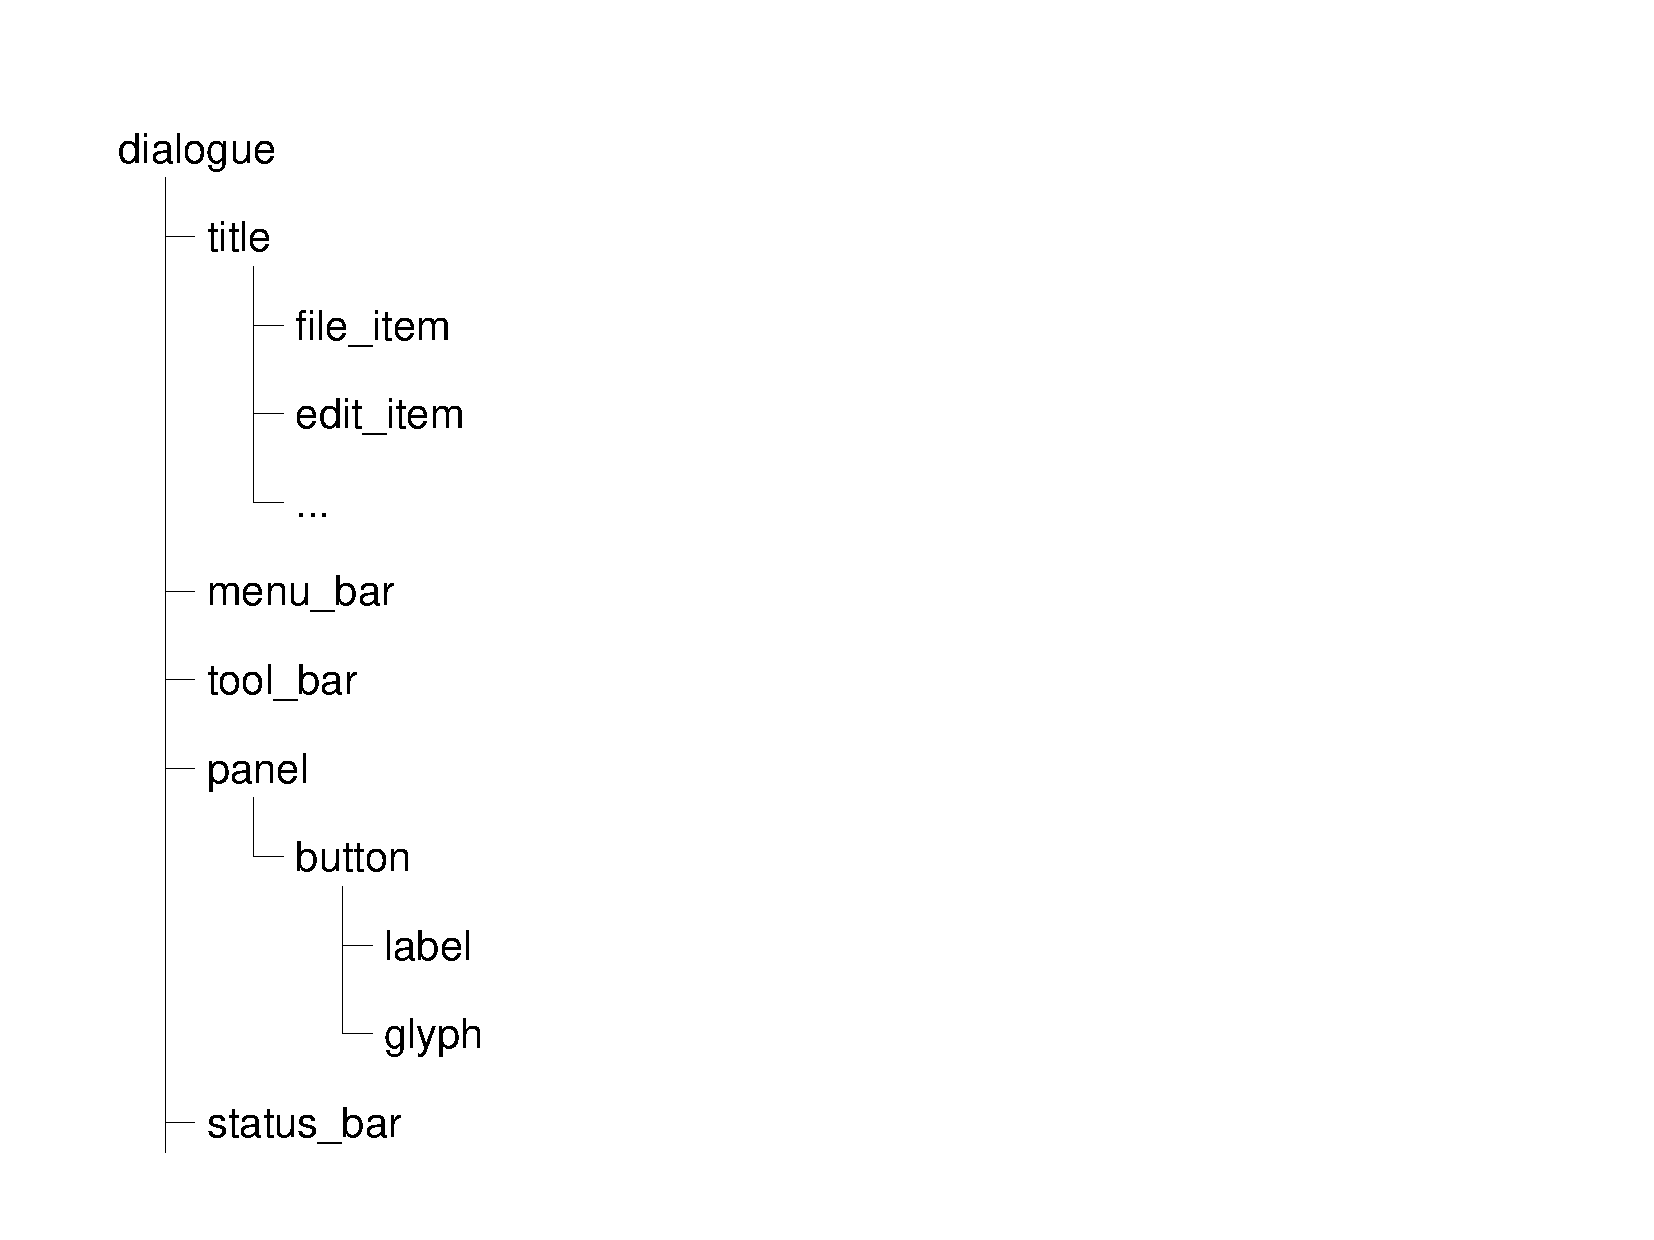
\includegraphics[scale=0.3,angle=-90]{graphic/md.pdf}
        \caption{CYBOL Model Diagram (MD) Proposal}
        \label{md_figure}
    \end{center}
\end{figure}

The MD (figure \ref{md_figure}) displays the runtime models that were
instantiated with knowledge templates providing the initial values. Again, the
parts of the graphical dialogue of figure \ref{editor_figure} are used in it.

\begin{figure}[ht]
    \begin{center}
        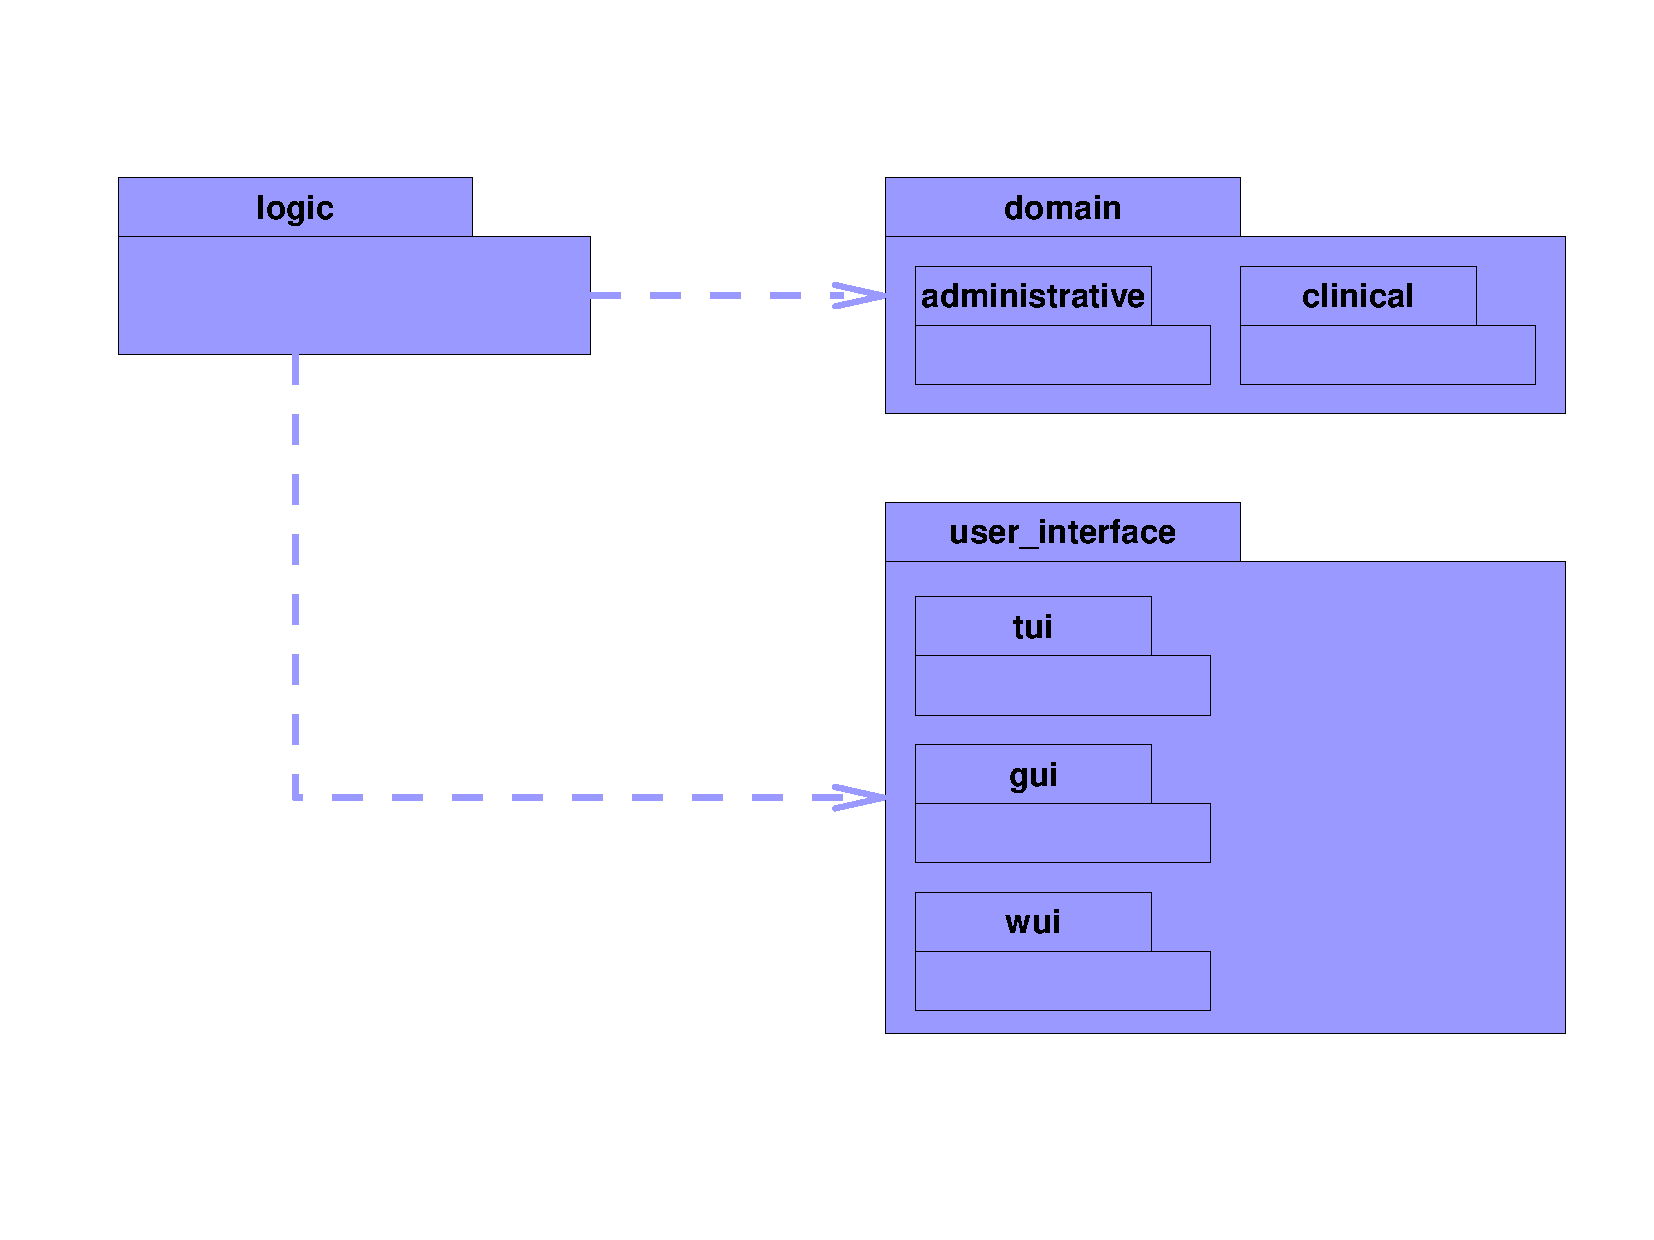
\includegraphics[scale=0.3,angle=-90]{graphic/od.pdf}
        \caption{CYBOL Organisation Diagram (OD) Proposal}
        \label{od_figure}
    \end{center}
\end{figure}

The OD (figure \ref{od_figure}) shows packages into which CYBOL knowledge
templates may be organised. Packages do normally correspond to directories on
file system level. The figure contains a \emph{domain} package consisting of
two sub packages, one containing knowledge templates for \emph{administrative}
patient data and the other holding templates for \emph{clinical} data of a
patient. Also, there is a \emph{User Interface} (UI) package containing three
sub packages, for: \emph{Textual UI} (TUI), \emph{Graphical UI} (GUI) and
\emph{Web UI} (WUI). Both, \emph{domain-} as well as \emph{user\_interface}
packages may be accessed from the operations residing in the \emph{logic}
package.

\begin{figure}[ht]
    \begin{center}
        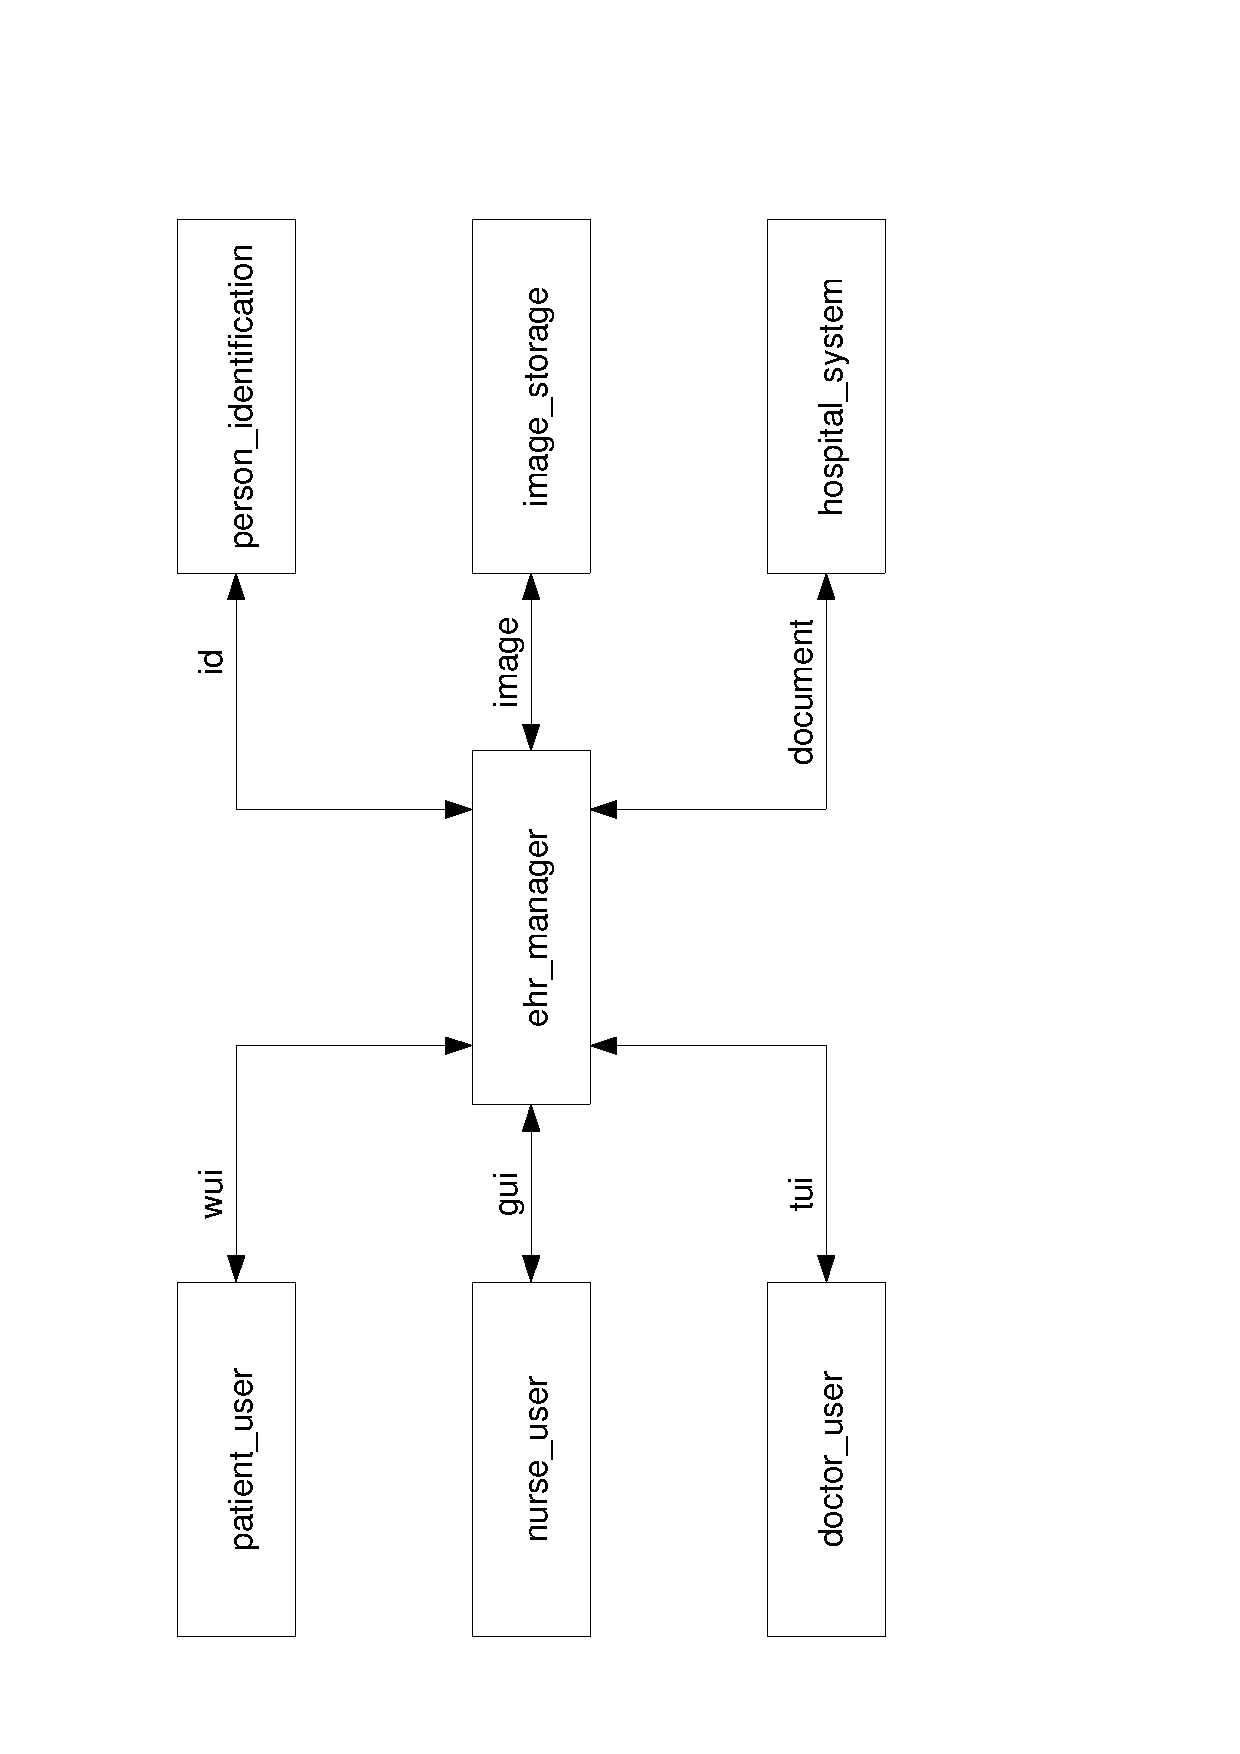
\includegraphics[scale=0.3,angle=-90]{graphic/cd.pdf}
        \caption{CYBOL Communication Diagram (CD) Proposal}
        \label{cd_figure}
    \end{center}
\end{figure}

The CD (figure \ref{cd_figure}), finally, shows a number of independent systems
communicating with each other. An \emph{Electronic Health Record} (EHR) manager
application may be found in the center of the figure. Patients communicate with
it using a WUI; nurses using a GUI and doctors using a TUI (for better
performance). A patient gets identified by asking a \emph{person\_identification}
service. Documents may be exchanged with a \emph{hospital\_system} and images
with a special \emph{image\_storage} system.

Besides these essential diagrams, additional ones may be used, of course. UML
diagrams like the AD, SD or TiD assist in modelling the flow of actions, that
is sequences of logic operations over time. Their ability to refine actions in
another level of granularity is of special interest. When removing the objects
bundled with method calls, they are well suitable for CYBOL. They use different
graphical elements, but in the end would store their knowledge in the same
templates. The transitions between different states of the runtime knowledge
tree over time are what the SMD wants to display. It may well be used with
CYBOL. But not only an application's behaviour over time is of interest, the
positions and expansions of its elements in space are as well important. This
mostly affects the design of user interfaces, graphical or textual. Designers
for these are therefore added to the list of useful diagrams. The usefulness of
feature model diagrams (section \ref{feature_model_heading}) for expressing
constraints that branches of the knowledge tree impose on each other could not
be investigated in this work, as this would break its frame.

Since CYBOL files contain all knowledge that is needed to define a complete
application system, the generation or parsing of classical source code is not
needed anymore, as chapter \ref{review_heading} will mention again. Therefore,
CYBOL knowledge design tools do only have to provide scanner- and generator
functionality for CYBOL (in order to formalise the knowledge designed as
semi-formal diagrams), but not for implementation languages.
